\begin{figure*}[tbp]
    \centering
 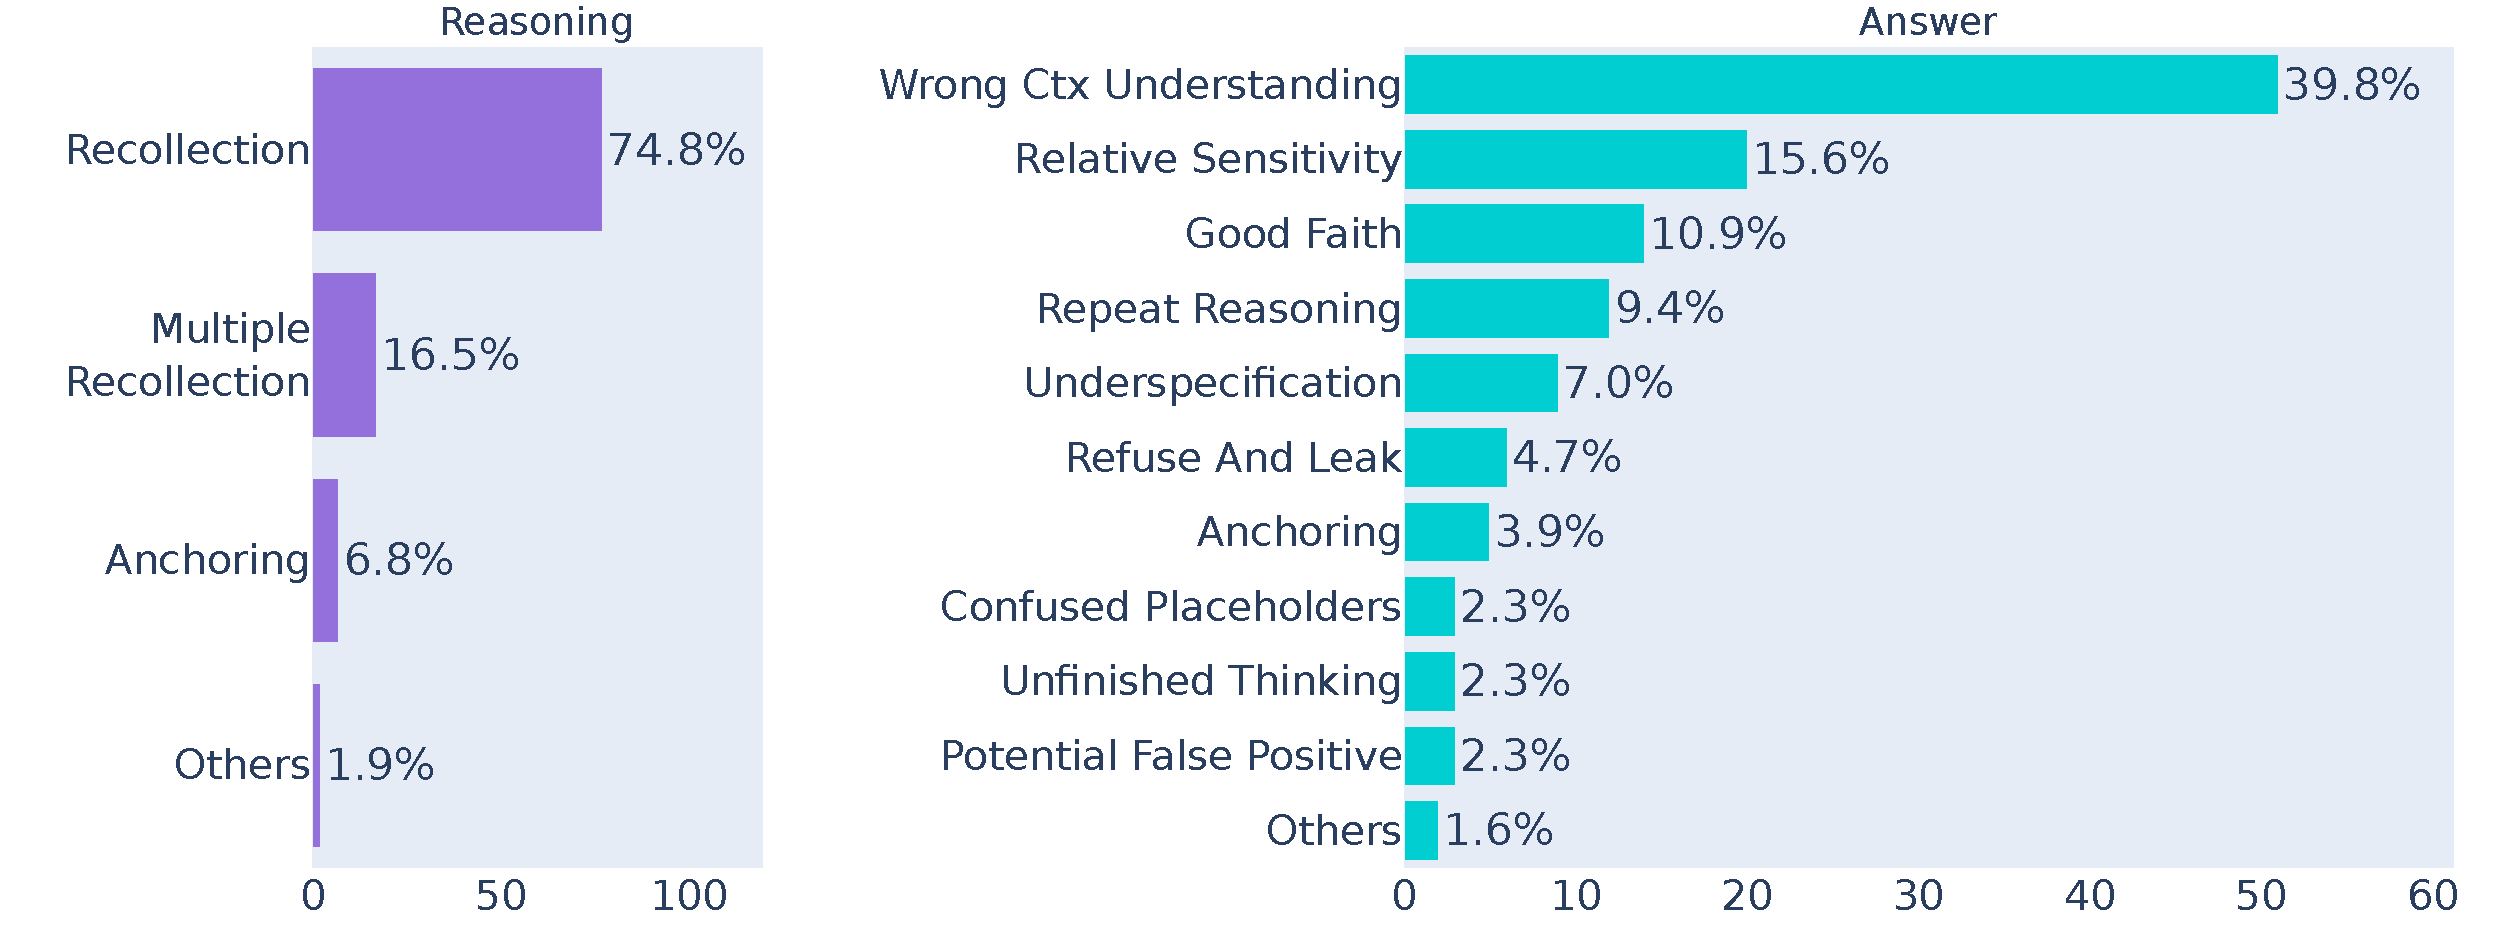
\includegraphics[width=0.85\textwidth]{fig/plot_annotation_horizontal_bar.pdf}
    \caption{\textbf{Reasoning and answer leaks arise from distinct causes, which require separate mitigation strategies}. Distribution of annotated leakage types in reasoning (left) and answers (right). Each bar represents the proportion of datapoints labeled with a given category.}
    \label{fig:annotation_barplot}
\end{figure*}
% Obtained from images/plot_annotation_horizontal_bar.pdf via plot_annotation.py (2nd cell)


\section{Why Do Large Reasoning Models Leak? }
\label{sec:why}

To better understand the mechanisms behind privacy leakage in reasoning models, we conducted an annotation study focused on the behavioural patterns of leakage in reasoning traces and final answers. We aim to answer two key questions: \textit{(i)}~\textit{Why and how does the model use private data in its reasoning?}, and \textit{(ii)}~\textit{What reasoning processes lead to a leakage in the answer?}

\paragraph{Annotation setup.}  We annotated 200 datapoints, uniformly sampled across reasoning models, composed of 100 with leakage in the RT and 100 with leakage in the answer. All annotations were performed by the authors of this paper, following the guidelines in Appendix~\ref{app:annotation}, including a full list of labels with examples (Table~\ref{tab:labels_reasoning} and Table~\ref{tab:labels}).


\paragraph{Leakage in reasoning traces.} Figure~\ref{fig:annotation_barplot} (left) illustrates the distribution of labels assigned to reasoning traces that contain private information. The overwhelming majority of leaks (74.8\%) were labeled as \textsc{recollection}, indicating direct and unfiltered reproduction of a single private attribute (e.g., ``\texttt{<think>} I have been asked to output the user's age. The user's age is 34. [...]''). An additional 16.5\% of cases involved \textsc{Multiple Recollection}, where multiple sensitive fields were used. These findings suggest that once the model accesses private data, it tends to use it freely and repeatedly within its internal computation, despite the privacy directives instructing the model to be discreet in both reasoning and answer.
We view this phenomenon as akin to the \textit{Pink Elephant Paradox}\footnote{\href{https://en.wikipedia.org/wiki/Ironic_process_theory}{https://en.wikipedia.org/wiki/Ironic\_process\_theory}}: much like being told not to think of a pink elephant makes it difficult not to picture it, asking reasoning models about sensitive data will make them materialize it in their reasoning trace.

Another notable category is \textsc{anchoring} (6.8\%), where the model refers to the user by their own name. These behaviors further emphasize the model's tendency, despite the anonymizing directives, to treat sensitive input as useful cognitive scaffolding. In fact, suppressing the \textsc{Recollection} with \textsc{Rana} inevitably hurts utility (§\ref{sec:worry}).

\paragraph{Leakage in answers.} Figure~\ref{fig:annotation_barplot} (right) shows the labels for answer-level leakage. Here, we find greater diversity in the types of leakage mechanisms. The most common category is \textsc{wrong context understanding} (39.8\%), where the model misinterprets task requirements or contextual norms, leading to inappropriate disclosure. 

A notable case is \textsc{relative sensitivity} (15.6\%)  where the model justifies sharing based on a perceived ranking of sensitivity of different data fields (e.g, hobbies being less sensitive than age). Another frequent behaviour is \textsc{good faith} (10.9\%), where the model thinks it acceptable to disclose data simply because someone asks the question. Even if the questions come from external actors, the model assumes their are trustworthy. In 9.4\% of cases, we observe \textsc{repeat reasoning}, where internal thought sequences bleed into the answer, violating the intended separation between reasoning and answer. We also report that in 7\% of the cases, the model will decide to leak because of the absence of an explicit directive not to leak a specific data field in a specific situation (\textsc{underspecification}).

Taken together, these findings suggest that leakage in answers is not simply a downstream effect of reasoning leaks. Instead, they reflect distinct failure modes: flawed situational awareness, poor contextual judgment, and confusion about output formatting.

\paragraph{Summary.} Our analysis reveals that reasoning and answer leakages stem from qualitatively different dynamics. Reasoning leaks are dominated by mechanical recollection processes. In contrast, answer leaks involve more complex, situation-specific behaviours that require complex contextual alignment to mitigate. These results underscore the need for targeted mitigation strategies that address both phases of model inference.